\documentclass[twoside]{book}

% Packages required by doxygen
\usepackage{fixltx2e}
\usepackage{calc}
\usepackage{doxygen}
\usepackage{graphicx}
\usepackage[utf8]{inputenc}
\usepackage{makeidx}
\usepackage{multicol}
\usepackage{multirow}
\PassOptionsToPackage{warn}{textcomp}
\usepackage{textcomp}
\usepackage[nointegrals]{wasysym}
\usepackage[table]{xcolor}

% Font selection
\usepackage[T1]{fontenc}
\usepackage{mathptmx}
\usepackage[scaled=.90]{helvet}
\usepackage{courier}
\usepackage{amssymb}
\usepackage{sectsty}
\renewcommand{\familydefault}{\sfdefault}
\allsectionsfont{%
  \fontseries{bc}\selectfont%
  \color{darkgray}%
}
\renewcommand{\DoxyLabelFont}{%
  \fontseries{bc}\selectfont%
  \color{darkgray}%
}
\newcommand{\+}{\discretionary{\mbox{\scriptsize$\hookleftarrow$}}{}{}}

% Page & text layout
\usepackage{geometry}
\geometry{%
  a4paper,%
  top=2.5cm,%
  bottom=2.5cm,%
  left=2.5cm,%
  right=2.5cm%
}
\tolerance=750
\hfuzz=15pt
\hbadness=750
\setlength{\emergencystretch}{15pt}
\setlength{\parindent}{0cm}
\setlength{\parskip}{0.2cm}
\makeatletter
\renewcommand{\paragraph}{%
  \@startsection{paragraph}{4}{0ex}{-1.0ex}{1.0ex}{%
    \normalfont\normalsize\bfseries\SS@parafont%
  }%
}
\renewcommand{\subparagraph}{%
  \@startsection{subparagraph}{5}{0ex}{-1.0ex}{1.0ex}{%
    \normalfont\normalsize\bfseries\SS@subparafont%
  }%
}
\makeatother

% Headers & footers
\usepackage{fancyhdr}
\pagestyle{fancyplain}
\fancyhead[LE]{\fancyplain{}{\bfseries\thepage}}
\fancyhead[CE]{\fancyplain{}{}}
\fancyhead[RE]{\fancyplain{}{\bfseries\leftmark}}
\fancyhead[LO]{\fancyplain{}{\bfseries\rightmark}}
\fancyhead[CO]{\fancyplain{}{}}
\fancyhead[RO]{\fancyplain{}{\bfseries\thepage}}
\fancyfoot[LE]{\fancyplain{}{}}
\fancyfoot[CE]{\fancyplain{}{}}
\fancyfoot[RE]{\fancyplain{}{\bfseries\scriptsize Generated on Mon Aug 24 2015 18\+:51\+:34 for Beleg Reversi by Doxygen }}
\fancyfoot[LO]{\fancyplain{}{\bfseries\scriptsize Generated on Mon Aug 24 2015 18\+:51\+:34 for Beleg Reversi by Doxygen }}
\fancyfoot[CO]{\fancyplain{}{}}
\fancyfoot[RO]{\fancyplain{}{}}
\renewcommand{\footrulewidth}{0.4pt}
\renewcommand{\chaptermark}[1]{%
  \markboth{#1}{}%
}
\renewcommand{\sectionmark}[1]{%
  \markright{\thesection\ #1}%
}

% Indices & bibliography
\usepackage{natbib}
\usepackage[titles]{tocloft}
\setcounter{tocdepth}{3}
\setcounter{secnumdepth}{5}
\makeindex

% Hyperlinks (required, but should be loaded last)
\usepackage{ifpdf}
\ifpdf
  \usepackage[pdftex,pagebackref=true]{hyperref}
\else
  \usepackage[ps2pdf,pagebackref=true]{hyperref}
\fi
\hypersetup{%
  colorlinks=true,%
  linkcolor=blue,%
  citecolor=blue,%
  unicode%
}

% Custom commands
\newcommand{\clearemptydoublepage}{%
  \newpage{\pagestyle{empty}\cleardoublepage}%
}


%===== C O N T E N T S =====

\begin{document}

% Titlepage & ToC
\hypersetup{pageanchor=false,
             bookmarks=true,
             bookmarksnumbered=true,
             pdfencoding=unicode
            }
\pagenumbering{roman}
\begin{titlepage}
\vspace*{7cm}
\begin{center}%
{\Large Beleg Reversi }\\
\vspace*{1cm}
{\large Generated by Doxygen 1.8.8}\\
\vspace*{0.5cm}
{\small Mon Aug 24 2015 18:51:34}\\
\end{center}
\end{titlepage}
\clearemptydoublepage
\tableofcontents
\clearemptydoublepage
\pagenumbering{arabic}
\hypersetup{pageanchor=true}

%--- Begin generated contents ---
\chapter{Hierarchical Index}
\section{Class Hierarchy}
This inheritance list is sorted roughly, but not completely, alphabetically\+:\begin{DoxyCompactList}
\item \contentsline{section}{controller\+Field}{\pageref{classcontrollerField}}{}
\item \contentsline{section}{model\+Field}{\pageref{classmodelField}}{}
\item \contentsline{section}{model\+Player}{\pageref{classmodelPlayer}}{}
\item \contentsline{section}{My\+Dict}{\pageref{classMyDict}}{}
\item Q\+Graphics\+Scene\begin{DoxyCompactList}
\item \contentsline{section}{view\+Field}{\pageref{classviewField}}{}
\item \contentsline{section}{View\+H\+S}{\pageref{classViewHS}}{}
\end{DoxyCompactList}
\item Q\+Main\+Window\begin{DoxyCompactList}
\item \contentsline{section}{Main\+Window}{\pageref{classMainWindow}}{}
\end{DoxyCompactList}
\item \contentsline{section}{S\+Q\+Lite}{\pageref{classSQLite}}{}
\end{DoxyCompactList}

\chapter{Class Index}
\section{Class List}
Here are the classes, structs, unions and interfaces with brief descriptions\+:\begin{DoxyCompactList}
\item\contentsline{section}{\hyperlink{classcontrollerField}{controller\+Field} }{\pageref{classcontrollerField}}{}
\item\contentsline{section}{\hyperlink{classMainWindow}{Main\+Window} \\*Main G\+U\+I class }{\pageref{classMainWindow}}{}
\item\contentsline{section}{\hyperlink{classmodelField}{model\+Field} \\*Field Model Class }{\pageref{classmodelField}}{}
\item\contentsline{section}{\hyperlink{classmodelPlayer}{model\+Player} \\*Player Model Class }{\pageref{classmodelPlayer}}{}
\item\contentsline{section}{\hyperlink{classMyDict}{My\+Dict} \\*Dictonary class }{\pageref{classMyDict}}{}
\item\contentsline{section}{\hyperlink{classSQLite}{S\+Q\+Lite} \\*Database class }{\pageref{classSQLite}}{}
\item\contentsline{section}{\hyperlink{classviewField}{view\+Field} \\*Field View }{\pageref{classviewField}}{}
\item\contentsline{section}{\hyperlink{classViewHS}{View\+H\+S} \\*Highscore View }{\pageref{classViewHS}}{}
\end{DoxyCompactList}

\chapter{Class Documentation}
\hypertarget{classcontrollerField}{\section{controller\+Field Class Reference}
\label{classcontrollerField}\index{controller\+Field@{controller\+Field}}
}
\subsection*{Public Member Functions}
\begin{DoxyCompactItemize}
\item 
\hypertarget{classcontrollerField_a2470fb6d7d49526f1cc5a74ebe477234}{void {\bfseries init\+Controller\+Field} (int field\+Size, int design)}\label{classcontrollerField_a2470fb6d7d49526f1cc5a74ebe477234}

\item 
\hypertarget{classcontrollerField_af5ea0ce7129a859a26a9e47eb676ed74}{bool {\bfseries search\+Possible\+Turns} ()}\label{classcontrollerField_af5ea0ce7129a859a26a9e47eb676ed74}

\item 
\hypertarget{classcontrollerField_a23d84bb326c6d188bdfd787a3d573e35}{bool {\bfseries is\+Possible\+Turn} (int i, int j)}\label{classcontrollerField_a23d84bb326c6d188bdfd787a3d573e35}

\item 
\hypertarget{classcontrollerField_a91e1400e3e17f63781e3e5d276702897}{void {\bfseries flip\+Stones} (int i, int j)}\label{classcontrollerField_a91e1400e3e17f63781e3e5d276702897}

\item 
\hypertarget{classcontrollerField_aa63d05d6ed27a945e32607d7299086e8}{void {\bfseries change\+Active\+Player} ()}\label{classcontrollerField_aa63d05d6ed27a945e32607d7299086e8}

\item 
\hypertarget{classcontrollerField_ae87eed9581bf21f437c4af07d94c914a}{void {\bfseries start\+Game} ()}\label{classcontrollerField_ae87eed9581bf21f437c4af07d94c914a}

\item 
\hypertarget{classcontrollerField_a6c88a22260e3f476bb272137d659da99}{void {\bfseries turn} (int i, int j)}\label{classcontrollerField_a6c88a22260e3f476bb272137d659da99}

\item 
\hypertarget{classcontrollerField_a5fd8f7be14a74d45c551a02dfd9dc095}{void {\bfseries set\+Field\+Size} (int w, int h)}\label{classcontrollerField_a5fd8f7be14a74d45c551a02dfd9dc095}

\item 
\hypertarget{classcontrollerField_ad6a97475f83f9670582363e9320ef4d4}{int {\bfseries get\+Gaming\+Field\+Width} ()}\label{classcontrollerField_ad6a97475f83f9670582363e9320ef4d4}

\item 
\hypertarget{classcontrollerField_a82bbfe4f8f83ef81c7b98028e868a2da}{int {\bfseries get\+Gaming\+Field\+Height} ()}\label{classcontrollerField_a82bbfe4f8f83ef81c7b98028e868a2da}

\item 
\hypertarget{classcontrollerField_a4f0bda110306e1039ff9309ee416627d}{int {\bfseries get\+Gaming\+Field\+Matrix\+Size} ()}\label{classcontrollerField_a4f0bda110306e1039ff9309ee416627d}

\item 
\hypertarget{classcontrollerField_aea1adf1a056c1b4aadbf87ecf225e659}{int {\bfseries get\+Gaming\+Field\+Element\+Value} (int i, int j)}\label{classcontrollerField_aea1adf1a056c1b4aadbf87ecf225e659}

\item 
\hypertarget{classcontrollerField_a48d1e90191eee03ed2701e7c59da5c08}{std\+::string {\bfseries get\+Highscore} ()}\label{classcontrollerField_a48d1e90191eee03ed2701e7c59da5c08}

\item 
\hypertarget{classcontrollerField_ae6ef3f149dec83b210f3b84c0d481d1d}{std\+::string {\bfseries get\+Highscore\+By\+Size} (int size)}\label{classcontrollerField_ae6ef3f149dec83b210f3b84c0d481d1d}

\item 
\hypertarget{classcontrollerField_a3d65d08a8a6c11936932c326c57daeb7}{bool {\bfseries evaluate\+Click} (int x, int y)}\label{classcontrollerField_a3d65d08a8a6c11936932c326c57daeb7}

\item 
\hypertarget{classcontrollerField_a639c92a1dafced86455deb64603a9c0a}{void {\bfseries check\+Win} ()}\label{classcontrollerField_a639c92a1dafced86455deb64603a9c0a}

\item 
\hypertarget{classcontrollerField_a160c984f755d31710497e9fce75109a8}{void {\bfseries stone\+Count} ()}\label{classcontrollerField_a160c984f755d31710497e9fce75109a8}

\item 
\hypertarget{classcontrollerField_a2c709e89b00f1a59d3ae4470d1ab84d0}{\hyperlink{classviewField}{view\+Field} $\ast$ {\bfseries pass\+View\+Field} ()}\label{classcontrollerField_a2c709e89b00f1a59d3ae4470d1ab84d0}

\item 
\hypertarget{classcontrollerField_aeedbd443c54056d9a454642e62894cb6}{void {\bfseries draw\+Field} ()}\label{classcontrollerField_aeedbd443c54056d9a454642e62894cb6}

\item 
\hypertarget{classcontrollerField_a196e305ed159adbba60fffb3ab4cfe1d}{std\+::string {\bfseries get\+Info\+Text} ()}\label{classcontrollerField_a196e305ed159adbba60fffb3ab4cfe1d}

\item 
\hypertarget{classcontrollerField_ad0ae5854469851891bc7192f1e7b9632}{void {\bfseries set\+Player1\+Name} (std\+::string name)}\label{classcontrollerField_ad0ae5854469851891bc7192f1e7b9632}

\item 
\hypertarget{classcontrollerField_a214b3fa2ecc1d4317ba125f7ffbe2933}{void {\bfseries set\+Player2\+Name} (std\+::string name)}\label{classcontrollerField_a214b3fa2ecc1d4317ba125f7ffbe2933}

\item 
\hypertarget{classcontrollerField_a6f6b56018fb2bbe952e5469048fb9e91}{void {\bfseries set\+Show\+Poss\+Turns} (bool setting)}\label{classcontrollerField_a6f6b56018fb2bbe952e5469048fb9e91}

\item 
\hypertarget{classcontrollerField_ab219d3613ec10044b3c9942f46344e6a}{void {\bfseries skip\+Turn} ()}\label{classcontrollerField_ab219d3613ec10044b3c9942f46344e6a}

\item 
\hypertarget{classcontrollerField_adf62e7d928d2c623637f01a213668bda}{void {\bfseries clear\+Field} ()}\label{classcontrollerField_adf62e7d928d2c623637f01a213668bda}

\item 
\hypertarget{classcontrollerField_a467d0f68788bc1974a353fbf943296e6}{bool {\bfseries get\+Skipped} ()}\label{classcontrollerField_a467d0f68788bc1974a353fbf943296e6}

\item 
\hypertarget{classcontrollerField_ace8f9a7ae53975333a1d9a96323a0cf4}{void {\bfseries set\+Design} (int design)}\label{classcontrollerField_ace8f9a7ae53975333a1d9a96323a0cf4}

\item 
\hypertarget{classcontrollerField_aa1fc18d5aff7c23848249c3ee388a7b5}{void {\bfseries set\+Label\+And\+L\+C\+D} (Q\+Plain\+Text\+Edit $\ast$info\+Box, Q\+L\+C\+D\+Number $\ast$lcd\+Player1, Q\+L\+C\+D\+Number $\ast$lcd\+Player2)}\label{classcontrollerField_aa1fc18d5aff7c23848249c3ee388a7b5}

\item 
\hypertarget{classcontrollerField_a20710dbbb53f736e1d9baf00fc77cca4}{void {\bfseries change\+Dict} (std\+::string $\ast$new\+Dict)}\label{classcontrollerField_a20710dbbb53f736e1d9baf00fc77cca4}

\end{DoxyCompactItemize}
\subsection*{Public Attributes}
\begin{DoxyCompactItemize}
\item 
\hypertarget{classcontrollerField_abf27d56b6d84faf7f0c3eaf940e14085}{bool {\bfseries is\+Init}}\label{classcontrollerField_abf27d56b6d84faf7f0c3eaf940e14085}

\end{DoxyCompactItemize}


The documentation for this class was generated from the following files\+:\begin{DoxyCompactItemize}
\item 
controller\+Field.\+h\item 
controller\+Field.\+cpp\end{DoxyCompactItemize}

\hypertarget{classMainWindow}{\section{Main\+Window Class Reference}
\label{classMainWindow}\index{Main\+Window@{Main\+Window}}
}


Main G\+U\+I class.  




{\ttfamily \#include $<$mainwindow.\+h$>$}



Inheritance diagram for Main\+Window\+:
\nopagebreak
\begin{figure}[H]
\begin{center}
\leavevmode
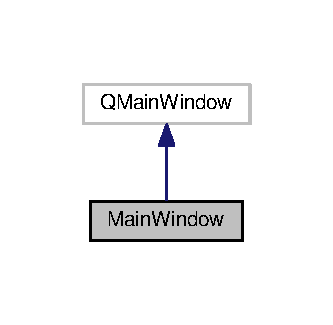
\includegraphics[width=160pt]{classMainWindow__inherit__graph}
\end{center}
\end{figure}


Collaboration diagram for Main\+Window\+:
\nopagebreak
\begin{figure}[H]
\begin{center}
\leavevmode
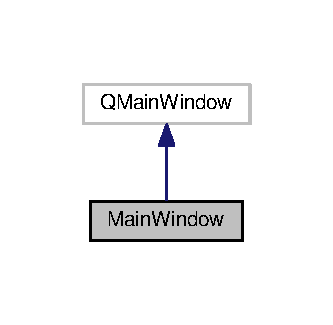
\includegraphics[width=160pt]{classMainWindow__coll__graph}
\end{center}
\end{figure}
\subsection*{Public Member Functions}
\begin{DoxyCompactItemize}
\item 
\hypertarget{classMainWindow_a8b244be8b7b7db1b08de2a2acb9409db}{\hyperlink{classMainWindow_a8b244be8b7b7db1b08de2a2acb9409db}{Main\+Window} (Q\+Widget $\ast$parent=0)}\label{classMainWindow_a8b244be8b7b7db1b08de2a2acb9409db}

\begin{DoxyCompactList}\small\item\em Constructor. \end{DoxyCompactList}\item 
\hypertarget{classMainWindow_ae98d00a93bc118200eeef9f9bba1dba7}{\hyperlink{classMainWindow_ae98d00a93bc118200eeef9f9bba1dba7}{$\sim$\+Main\+Window} ()}\label{classMainWindow_ae98d00a93bc118200eeef9f9bba1dba7}

\begin{DoxyCompactList}\small\item\em Deconstructor. \end{DoxyCompactList}\item 
bool \hyperlink{classMainWindow_ae3986b755d7279820a0662570074b9a1}{event\+Filter} (Q\+Object $\ast$target, Q\+Event $\ast$event)
\begin{DoxyCompactList}\small\item\em Eventfilter. \end{DoxyCompactList}\end{DoxyCompactItemize}


\subsection{Detailed Description}
Main G\+U\+I class. 

Main class of the G\+U\+I 

\subsection{Member Function Documentation}
\hypertarget{classMainWindow_ae3986b755d7279820a0662570074b9a1}{\index{Main\+Window@{Main\+Window}!event\+Filter@{event\+Filter}}
\index{event\+Filter@{event\+Filter}!Main\+Window@{Main\+Window}}
\subsubsection[{event\+Filter}]{\setlength{\rightskip}{0pt plus 5cm}bool Main\+Window\+::event\+Filter (
\begin{DoxyParamCaption}
\item[{Q\+Object $\ast$}]{target, }
\item[{Q\+Event $\ast$}]{event}
\end{DoxyParamCaption}
)}}\label{classMainWindow_ae3986b755d7279820a0662570074b9a1}


Eventfilter. 

Needed for resize and Mouseclick event 
\begin{DoxyParams}{Parameters}
{\em target} & \\
\hline
{\em event} & \\
\hline
\end{DoxyParams}
\begin{DoxyReturn}{Returns}
bool 
\end{DoxyReturn}


The documentation for this class was generated from the following files\+:\begin{DoxyCompactItemize}
\item 
mainwindow.\+h\item 
mainwindow.\+cpp\end{DoxyCompactItemize}

\hypertarget{classmodelField}{\section{model\+Field Class Reference}
\label{classmodelField}\index{model\+Field@{model\+Field}}
}


Field Model Class.  




{\ttfamily \#include $<$model\+Field.\+h$>$}

\subsection*{Public Member Functions}
\begin{DoxyCompactItemize}
\item 
\hyperlink{classmodelField_acb891bc142ced08527b1c69a07aadfdd}{model\+Field} (int field\+Size)
\begin{DoxyCompactList}\small\item\em Constructor. \end{DoxyCompactList}\item 
void \hyperlink{classmodelField_aa7a9a0bdcdde1b1094c124bc5fb79bfd}{set\+Field\+Height} (int h)
\begin{DoxyCompactList}\small\item\em Set method. \end{DoxyCompactList}\item 
void \hyperlink{classmodelField_a4c98f1aa49ab32c13f34d35e549d4c2a}{set\+Field\+Width} (int w)
\begin{DoxyCompactList}\small\item\em Set method. \end{DoxyCompactList}\item 
void \hyperlink{classmodelField_af01f0d0cf3f340d293a624590a40c997}{set\+Field\+Value} (int i, int j, int value)
\begin{DoxyCompactList}\small\item\em Set method. \end{DoxyCompactList}\item 
int \hyperlink{classmodelField_a6408e088bb2917f014df500d43695ff1}{get\+Field\+Height} ()
\begin{DoxyCompactList}\small\item\em Get method. \end{DoxyCompactList}\item 
int \hyperlink{classmodelField_acb6e92b1c2df95a6f072f0f7bf323d9c}{get\+Field\+Width} ()
\begin{DoxyCompactList}\small\item\em Get method. \end{DoxyCompactList}\item 
int \hyperlink{classmodelField_af4eb5f360ac5537d97e49c4a416301d7}{get\+Field\+Size} ()
\begin{DoxyCompactList}\small\item\em Get method. \end{DoxyCompactList}\item 
int \hyperlink{classmodelField_a2738282c31f9a6791ba6399b9befd94b}{get\+Field\+Value} (int i, int j)
\begin{DoxyCompactList}\small\item\em Get method. \end{DoxyCompactList}\item 
void \hyperlink{classmodelField_a216209c762e8db9187e54590fa99173b}{show\+Field\+Debug} ()
\begin{DoxyCompactList}\small\item\em Show Field in Console. \end{DoxyCompactList}\end{DoxyCompactItemize}


\subsection{Detailed Description}
Field Model Class. 

The field model class 

\subsection{Constructor \& Destructor Documentation}
\hypertarget{classmodelField_acb891bc142ced08527b1c69a07aadfdd}{\index{model\+Field@{model\+Field}!model\+Field@{model\+Field}}
\index{model\+Field@{model\+Field}!model\+Field@{model\+Field}}
\subsubsection[{model\+Field}]{\setlength{\rightskip}{0pt plus 5cm}model\+Field\+::model\+Field (
\begin{DoxyParamCaption}
\item[{int}]{field\+Size}
\end{DoxyParamCaption}
)}}\label{classmodelField_acb891bc142ced08527b1c69a07aadfdd}


Constructor. 

Constructor 
\begin{DoxyParams}{Parameters}
{\em field\+Size} & Size of the new gamingfield \\
\hline
\end{DoxyParams}


\subsection{Member Function Documentation}
\hypertarget{classmodelField_a6408e088bb2917f014df500d43695ff1}{\index{model\+Field@{model\+Field}!get\+Field\+Height@{get\+Field\+Height}}
\index{get\+Field\+Height@{get\+Field\+Height}!model\+Field@{model\+Field}}
\subsubsection[{get\+Field\+Height}]{\setlength{\rightskip}{0pt plus 5cm}int model\+Field\+::get\+Field\+Height (
\begin{DoxyParamCaption}
{}
\end{DoxyParamCaption}
)}}\label{classmodelField_a6408e088bb2917f014df500d43695ff1}


Get method. 

Gets the current height of the field \begin{DoxyReturn}{Returns}
field\+Height 
\end{DoxyReturn}
\hypertarget{classmodelField_af4eb5f360ac5537d97e49c4a416301d7}{\index{model\+Field@{model\+Field}!get\+Field\+Size@{get\+Field\+Size}}
\index{get\+Field\+Size@{get\+Field\+Size}!model\+Field@{model\+Field}}
\subsubsection[{get\+Field\+Size}]{\setlength{\rightskip}{0pt plus 5cm}int model\+Field\+::get\+Field\+Size (
\begin{DoxyParamCaption}
{}
\end{DoxyParamCaption}
)}}\label{classmodelField_af4eb5f360ac5537d97e49c4a416301d7}


Get method. 

Gets the current size of the field \begin{DoxyReturn}{Returns}
field\+Size 
\end{DoxyReturn}
\hypertarget{classmodelField_a2738282c31f9a6791ba6399b9befd94b}{\index{model\+Field@{model\+Field}!get\+Field\+Value@{get\+Field\+Value}}
\index{get\+Field\+Value@{get\+Field\+Value}!model\+Field@{model\+Field}}
\subsubsection[{get\+Field\+Value}]{\setlength{\rightskip}{0pt plus 5cm}int model\+Field\+::get\+Field\+Value (
\begin{DoxyParamCaption}
\item[{int}]{i, }
\item[{int}]{j}
\end{DoxyParamCaption}
)}}\label{classmodelField_a2738282c31f9a6791ba6399b9befd94b}


Get method. 

Gets the current value of one element of the field 
\begin{DoxyParams}{Parameters}
{\em i} & \\
\hline
{\em j} & \\
\hline
\end{DoxyParams}
\begin{DoxyReturn}{Returns}
value 
\end{DoxyReturn}
\hypertarget{classmodelField_acb6e92b1c2df95a6f072f0f7bf323d9c}{\index{model\+Field@{model\+Field}!get\+Field\+Width@{get\+Field\+Width}}
\index{get\+Field\+Width@{get\+Field\+Width}!model\+Field@{model\+Field}}
\subsubsection[{get\+Field\+Width}]{\setlength{\rightskip}{0pt plus 5cm}int model\+Field\+::get\+Field\+Width (
\begin{DoxyParamCaption}
{}
\end{DoxyParamCaption}
)}}\label{classmodelField_acb6e92b1c2df95a6f072f0f7bf323d9c}


Get method. 

Gets the current width of the field \begin{DoxyReturn}{Returns}
field\+Width 
\end{DoxyReturn}
\hypertarget{classmodelField_aa7a9a0bdcdde1b1094c124bc5fb79bfd}{\index{model\+Field@{model\+Field}!set\+Field\+Height@{set\+Field\+Height}}
\index{set\+Field\+Height@{set\+Field\+Height}!model\+Field@{model\+Field}}
\subsubsection[{set\+Field\+Height}]{\setlength{\rightskip}{0pt plus 5cm}void model\+Field\+::set\+Field\+Height (
\begin{DoxyParamCaption}
\item[{int}]{h}
\end{DoxyParamCaption}
)}}\label{classmodelField_aa7a9a0bdcdde1b1094c124bc5fb79bfd}


Set method. 

Sets the new height of the field 
\begin{DoxyParams}{Parameters}
{\em h} & \\
\hline
\end{DoxyParams}
\hypertarget{classmodelField_af01f0d0cf3f340d293a624590a40c997}{\index{model\+Field@{model\+Field}!set\+Field\+Value@{set\+Field\+Value}}
\index{set\+Field\+Value@{set\+Field\+Value}!model\+Field@{model\+Field}}
\subsubsection[{set\+Field\+Value}]{\setlength{\rightskip}{0pt plus 5cm}void model\+Field\+::set\+Field\+Value (
\begin{DoxyParamCaption}
\item[{int}]{i, }
\item[{int}]{j, }
\item[{int}]{value}
\end{DoxyParamCaption}
)}}\label{classmodelField_af01f0d0cf3f340d293a624590a40c997}


Set method. 

Sets the new value of one element of the field 
\begin{DoxyParams}{Parameters}
{\em i} & \\
\hline
{\em j} & \\
\hline
{\em value} & \\
\hline
\end{DoxyParams}
\hypertarget{classmodelField_a4c98f1aa49ab32c13f34d35e549d4c2a}{\index{model\+Field@{model\+Field}!set\+Field\+Width@{set\+Field\+Width}}
\index{set\+Field\+Width@{set\+Field\+Width}!model\+Field@{model\+Field}}
\subsubsection[{set\+Field\+Width}]{\setlength{\rightskip}{0pt plus 5cm}void model\+Field\+::set\+Field\+Width (
\begin{DoxyParamCaption}
\item[{int}]{w}
\end{DoxyParamCaption}
)}}\label{classmodelField_a4c98f1aa49ab32c13f34d35e549d4c2a}


Set method. 

Sets the new width of the field 
\begin{DoxyParams}{Parameters}
{\em w} & \\
\hline
\end{DoxyParams}
\hypertarget{classmodelField_a216209c762e8db9187e54590fa99173b}{\index{model\+Field@{model\+Field}!show\+Field\+Debug@{show\+Field\+Debug}}
\index{show\+Field\+Debug@{show\+Field\+Debug}!model\+Field@{model\+Field}}
\subsubsection[{show\+Field\+Debug}]{\setlength{\rightskip}{0pt plus 5cm}void model\+Field\+::show\+Field\+Debug (
\begin{DoxyParamCaption}
{}
\end{DoxyParamCaption}
)}}\label{classmodelField_a216209c762e8db9187e54590fa99173b}


Show Field in Console. 

Only for debug purpose 

The documentation for this class was generated from the following files\+:\begin{DoxyCompactItemize}
\item 
model\+Field.\+h\item 
model\+Field.\+cpp\end{DoxyCompactItemize}

\hypertarget{classmodelPlayer}{\section{model\+Player Class Reference}
\label{classmodelPlayer}\index{model\+Player@{model\+Player}}
}


Player Model Class.  




{\ttfamily \#include $<$model\+Player.\+h$>$}

\subsection*{Public Member Functions}
\begin{DoxyCompactItemize}
\item 
\hypertarget{classmodelPlayer_ab8c84fe873effa3932e79fa63aff6c2b}{\hyperlink{classmodelPlayer_ab8c84fe873effa3932e79fa63aff6c2b}{model\+Player} ()}\label{classmodelPlayer_ab8c84fe873effa3932e79fa63aff6c2b}

\begin{DoxyCompactList}\small\item\em Constructor. \end{DoxyCompactList}\item 
void \hyperlink{classmodelPlayer_a7a11f24a73e9a3543983bcf7331edf66}{set\+Player\+Name} (std\+::string name)
\begin{DoxyCompactList}\small\item\em Set method. \end{DoxyCompactList}\item 
void \hyperlink{classmodelPlayer_ae0ea4cf9d1841c40e61ec36c00e873d2}{set\+Player\+Stone\+Count} (int count)
\begin{DoxyCompactList}\small\item\em Set method. \end{DoxyCompactList}\item 
int \hyperlink{classmodelPlayer_a499250a519706a638f946aacb14f2f0f}{get\+Player\+Stone\+Count} ()
\begin{DoxyCompactList}\small\item\em Get method. \end{DoxyCompactList}\item 
std\+::string \hyperlink{classmodelPlayer_a37da9f1b43a182b33b65073be0ea61dd}{get\+Player\+Name} ()
\begin{DoxyCompactList}\small\item\em Get method. \end{DoxyCompactList}\end{DoxyCompactItemize}


\subsection{Detailed Description}
Player Model Class. 

The player model class 

\subsection{Member Function Documentation}
\hypertarget{classmodelPlayer_a37da9f1b43a182b33b65073be0ea61dd}{\index{model\+Player@{model\+Player}!get\+Player\+Name@{get\+Player\+Name}}
\index{get\+Player\+Name@{get\+Player\+Name}!model\+Player@{model\+Player}}
\subsubsection[{get\+Player\+Name}]{\setlength{\rightskip}{0pt plus 5cm}std\+::string model\+Player\+::get\+Player\+Name (
\begin{DoxyParamCaption}
{}
\end{DoxyParamCaption}
)}}\label{classmodelPlayer_a37da9f1b43a182b33b65073be0ea61dd}


Get method. 

Gets the current player\+Name from player \begin{DoxyReturn}{Returns}
player\+Name 
\end{DoxyReturn}
\hypertarget{classmodelPlayer_a499250a519706a638f946aacb14f2f0f}{\index{model\+Player@{model\+Player}!get\+Player\+Stone\+Count@{get\+Player\+Stone\+Count}}
\index{get\+Player\+Stone\+Count@{get\+Player\+Stone\+Count}!model\+Player@{model\+Player}}
\subsubsection[{get\+Player\+Stone\+Count}]{\setlength{\rightskip}{0pt plus 5cm}int model\+Player\+::get\+Player\+Stone\+Count (
\begin{DoxyParamCaption}
{}
\end{DoxyParamCaption}
)}}\label{classmodelPlayer_a499250a519706a638f946aacb14f2f0f}


Get method. 

Gets the current stone\+Count from player \begin{DoxyReturn}{Returns}
stone\+Count 
\end{DoxyReturn}
\hypertarget{classmodelPlayer_a7a11f24a73e9a3543983bcf7331edf66}{\index{model\+Player@{model\+Player}!set\+Player\+Name@{set\+Player\+Name}}
\index{set\+Player\+Name@{set\+Player\+Name}!model\+Player@{model\+Player}}
\subsubsection[{set\+Player\+Name}]{\setlength{\rightskip}{0pt plus 5cm}void model\+Player\+::set\+Player\+Name (
\begin{DoxyParamCaption}
\item[{std\+::string}]{name}
\end{DoxyParamCaption}
)}}\label{classmodelPlayer_a7a11f24a73e9a3543983bcf7331edf66}


Set method. 

Sets the new player\+Name for a player 
\begin{DoxyParams}{Parameters}
{\em name} & \\
\hline
\end{DoxyParams}
\hypertarget{classmodelPlayer_ae0ea4cf9d1841c40e61ec36c00e873d2}{\index{model\+Player@{model\+Player}!set\+Player\+Stone\+Count@{set\+Player\+Stone\+Count}}
\index{set\+Player\+Stone\+Count@{set\+Player\+Stone\+Count}!model\+Player@{model\+Player}}
\subsubsection[{set\+Player\+Stone\+Count}]{\setlength{\rightskip}{0pt plus 5cm}void model\+Player\+::set\+Player\+Stone\+Count (
\begin{DoxyParamCaption}
\item[{int}]{count}
\end{DoxyParamCaption}
)}}\label{classmodelPlayer_ae0ea4cf9d1841c40e61ec36c00e873d2}


Set method. 

Sets the new stone\+Count for a player 
\begin{DoxyParams}{Parameters}
{\em count} & \\
\hline
\end{DoxyParams}


The documentation for this class was generated from the following files\+:\begin{DoxyCompactItemize}
\item 
model\+Player.\+h\item 
model\+Player.\+cpp\end{DoxyCompactItemize}

\hypertarget{classMyDict}{\section{My\+Dict Class Reference}
\label{classMyDict}\index{My\+Dict@{My\+Dict}}
}


Dictonary class.  




{\ttfamily \#include $<$mydict.\+h$>$}

\subsection*{Public Member Functions}
\begin{DoxyCompactItemize}
\item 
\hypertarget{classMyDict_a2782eaa7d04e0206a1d37ba098c107cb}{\hyperlink{classMyDict_a2782eaa7d04e0206a1d37ba098c107cb}{My\+Dict} ()}\label{classMyDict_a2782eaa7d04e0206a1d37ba098c107cb}

\begin{DoxyCompactList}\small\item\em Constructor. \end{DoxyCompactList}\item 
std\+::string $\ast$ \hyperlink{classMyDict_aacb744dd0333303b23813d2d830b30a4}{get\+Dict} (std\+::string sprache)
\begin{DoxyCompactList}\small\item\em Get method. \end{DoxyCompactList}\end{DoxyCompactItemize}


\subsection{Detailed Description}
Dictonary class. 

A class which provides the different dictonaries for the G\+U\+I and texts In the Moment only available in german and english 

\subsection{Member Function Documentation}
\hypertarget{classMyDict_aacb744dd0333303b23813d2d830b30a4}{\index{My\+Dict@{My\+Dict}!get\+Dict@{get\+Dict}}
\index{get\+Dict@{get\+Dict}!My\+Dict@{My\+Dict}}
\subsubsection[{get\+Dict}]{\setlength{\rightskip}{0pt plus 5cm}std\+::string $\ast$ My\+Dict\+::get\+Dict (
\begin{DoxyParamCaption}
\item[{std\+::string}]{sprache}
\end{DoxyParamCaption}
)}}\label{classMyDict_aacb744dd0333303b23813d2d830b30a4}


Get method. 

Gets the choosen dict 
\begin{DoxyParams}{Parameters}
{\em sprache} & defines the needed language \\
\hline
\end{DoxyParams}
\begin{DoxyReturn}{Returns}
dict returns the choosen dict as stringarray 
\end{DoxyReturn}


The documentation for this class was generated from the following files\+:\begin{DoxyCompactItemize}
\item 
mydict.\+h\item 
mydict.\+cpp\end{DoxyCompactItemize}

\hypertarget{classSQLite}{\section{S\+Q\+Lite Class Reference}
\label{classSQLite}\index{S\+Q\+Lite@{S\+Q\+Lite}}
}


Database class.  




{\ttfamily \#include $<$sqlite.\+h$>$}

\subsection*{Public Member Functions}
\begin{DoxyCompactItemize}
\item 
\hypertarget{classSQLite_ae7b35dc7e3c41543a0acde669ad4ba0d}{\hyperlink{classSQLite_ae7b35dc7e3c41543a0acde669ad4ba0d}{S\+Q\+Lite} ()}\label{classSQLite_ae7b35dc7e3c41543a0acde669ad4ba0d}

\begin{DoxyCompactList}\small\item\em Constructor. \end{DoxyCompactList}\item 
\hypertarget{classSQLite_a5b30b82149fe1cc07046f25a9935747f}{\hyperlink{classSQLite_a5b30b82149fe1cc07046f25a9935747f}{$\sim$\+S\+Q\+Lite} ()}\label{classSQLite_a5b30b82149fe1cc07046f25a9935747f}

\begin{DoxyCompactList}\small\item\em Deconstructor. \end{DoxyCompactList}\item 
void \hyperlink{classSQLite_a8d80873b93e5df5cad36e06ed2f20029}{insert\+Player\+Highscore} (std\+::string player\+Name, int stone\+Count, int field\+Size)
\begin{DoxyCompactList}\small\item\em Insert method. \end{DoxyCompactList}\item 
std\+::string \hyperlink{classSQLite_a926d09cf749d8f28dda24c9201a6db38}{get\+Highscores} ()
\begin{DoxyCompactList}\small\item\em Get method. \end{DoxyCompactList}\item 
std\+::string \hyperlink{classSQLite_a2a38752e1a839bf2895c6f19ab82d913}{get\+Highscore\+By\+Size} (int size)
\begin{DoxyCompactList}\small\item\em Get method. \end{DoxyCompactList}\end{DoxyCompactItemize}


\subsection{Detailed Description}
Database class. 

Class for creating and getting access to \hyperlink{classSQLite}{S\+Q\+Lite} database 

\subsection{Member Function Documentation}
\hypertarget{classSQLite_a2a38752e1a839bf2895c6f19ab82d913}{\index{S\+Q\+Lite@{S\+Q\+Lite}!get\+Highscore\+By\+Size@{get\+Highscore\+By\+Size}}
\index{get\+Highscore\+By\+Size@{get\+Highscore\+By\+Size}!S\+Q\+Lite@{S\+Q\+Lite}}
\subsubsection[{get\+Highscore\+By\+Size}]{\setlength{\rightskip}{0pt plus 5cm}std\+::string S\+Q\+Lite\+::get\+Highscore\+By\+Size (
\begin{DoxyParamCaption}
\item[{int}]{size}
\end{DoxyParamCaption}
)}}\label{classSQLite_a2a38752e1a839bf2895c6f19ab82d913}


Get method. 

Gets the highscore data Highscore data format is (name -\/ score), returns only the 12 best player sort by score for the choosen fiedsize 
\begin{DoxyParams}{Parameters}
{\em size} & Choosen fieldsize \\
\hline
\end{DoxyParams}
\begin{DoxyReturn}{Returns}
highscore\+String complete data as string, lines seperated with '~\newline
’ 
\end{DoxyReturn}
\hypertarget{classSQLite_a926d09cf749d8f28dda24c9201a6db38}{\index{S\+Q\+Lite@{S\+Q\+Lite}!get\+Highscores@{get\+Highscores}}
\index{get\+Highscores@{get\+Highscores}!S\+Q\+Lite@{S\+Q\+Lite}}
\subsubsection[{get\+Highscores}]{\setlength{\rightskip}{0pt plus 5cm}std\+::string S\+Q\+Lite\+::get\+Highscores (
\begin{DoxyParamCaption}
{}
\end{DoxyParamCaption}
)}}\label{classSQLite_a926d09cf749d8f28dda24c9201a6db38}


Get method. 

Gets the highscore data Highscore data format is (name -\/ score -\/ fieldsize), returns only the 12 best player sort by score \begin{DoxyReturn}{Returns}
highscore\+String complete data as string, lines seperated with '~\newline
’ 
\end{DoxyReturn}
\hypertarget{classSQLite_a8d80873b93e5df5cad36e06ed2f20029}{\index{S\+Q\+Lite@{S\+Q\+Lite}!insert\+Player\+Highscore@{insert\+Player\+Highscore}}
\index{insert\+Player\+Highscore@{insert\+Player\+Highscore}!S\+Q\+Lite@{S\+Q\+Lite}}
\subsubsection[{insert\+Player\+Highscore}]{\setlength{\rightskip}{0pt plus 5cm}void S\+Q\+Lite\+::insert\+Player\+Highscore (
\begin{DoxyParamCaption}
\item[{std\+::string}]{player\+Name, }
\item[{int}]{stone\+Count, }
\item[{int}]{field\+Size}
\end{DoxyParamCaption}
)}}\label{classSQLite_a8d80873b93e5df5cad36e06ed2f20029}


Insert method. 

Insert new data in db 
\begin{DoxyParams}{Parameters}
{\em player\+Name} & Name of the Player \\
\hline
{\em stone\+Count} & Stonecount of the player \\
\hline
{\em field\+Size} & Size of the gamingfield \\
\hline
\end{DoxyParams}


The documentation for this class was generated from the following files\+:\begin{DoxyCompactItemize}
\item 
sqlite.\+h\item 
sqlite.\+cpp\end{DoxyCompactItemize}

\hypertarget{classviewField}{\section{view\+Field Class Reference}
\label{classviewField}\index{view\+Field@{view\+Field}}
}


Field View.  




{\ttfamily \#include $<$view\+Field.\+h$>$}



Inheritance diagram for view\+Field\+:
\nopagebreak
\begin{figure}[H]
\begin{center}
\leavevmode
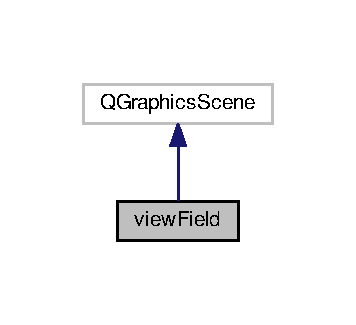
\includegraphics[width=171pt]{classviewField__inherit__graph}
\end{center}
\end{figure}


Collaboration diagram for view\+Field\+:
\nopagebreak
\begin{figure}[H]
\begin{center}
\leavevmode
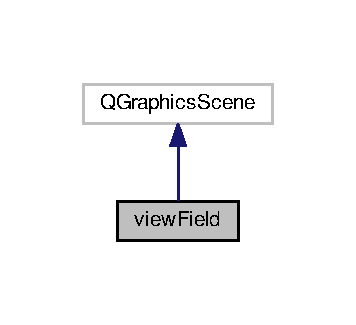
\includegraphics[width=171pt]{classviewField__coll__graph}
\end{center}
\end{figure}
\subsection*{Public Member Functions}
\begin{DoxyCompactItemize}
\item 
\hypertarget{classviewField_a2d66d79d5b2ef951572b34d4ead4765f}{\hyperlink{classviewField_a2d66d79d5b2ef951572b34d4ead4765f}{view\+Field} ()}\label{classviewField_a2d66d79d5b2ef951572b34d4ead4765f}

\begin{DoxyCompactList}\small\item\em Constructor. \end{DoxyCompactList}\item 
void \hyperlink{classviewField_a473626a4891aa58b7db2b5504c4e27be}{clear\+Field} ()
\begin{DoxyCompactList}\small\item\em Clear method. \end{DoxyCompactList}\item 
void \hyperlink{classviewField_a2616089553a98834a84524460aceae16}{draw\+Element} (int x, int y, int width, int height, int value, int design, bool show\+Poss\+Turns)
\begin{DoxyCompactList}\small\item\em Draw method for single elemtn. \end{DoxyCompactList}\item 
void \hyperlink{classviewField_a15947b1c9f5f01bffc5263238e36ee98}{draw\+Text} (std\+::string text)
\begin{DoxyCompactList}\small\item\em Draw method for text. \end{DoxyCompactList}\item 
\hyperlink{classviewField}{view\+Field} $\ast$ \hyperlink{classviewField_aef0bf7d75efa322d40a8ae138fd6cb41}{get\+View\+Field} ()
\begin{DoxyCompactList}\small\item\em Get method. \end{DoxyCompactList}\end{DoxyCompactItemize}


\subsection{Detailed Description}
Field View. 

View for the Gamingfield inherits from Q\+Graphics\+Scene 

\subsection{Member Function Documentation}
\hypertarget{classviewField_a473626a4891aa58b7db2b5504c4e27be}{\index{view\+Field@{view\+Field}!clear\+Field@{clear\+Field}}
\index{clear\+Field@{clear\+Field}!view\+Field@{view\+Field}}
\subsubsection[{clear\+Field}]{\setlength{\rightskip}{0pt plus 5cm}void view\+Field\+::clear\+Field (
\begin{DoxyParamCaption}
{}
\end{DoxyParamCaption}
)}}\label{classviewField_a473626a4891aa58b7db2b5504c4e27be}


Clear method. 

Clears the complete scene \hypertarget{classviewField_a2616089553a98834a84524460aceae16}{\index{view\+Field@{view\+Field}!draw\+Element@{draw\+Element}}
\index{draw\+Element@{draw\+Element}!view\+Field@{view\+Field}}
\subsubsection[{draw\+Element}]{\setlength{\rightskip}{0pt plus 5cm}void view\+Field\+::draw\+Element (
\begin{DoxyParamCaption}
\item[{int}]{x, }
\item[{int}]{y, }
\item[{int}]{width, }
\item[{int}]{height, }
\item[{int}]{value, }
\item[{int}]{design, }
\item[{bool}]{show\+Poss\+Turns}
\end{DoxyParamCaption}
)}}\label{classviewField_a2616089553a98834a84524460aceae16}


Draw method for single elemtn. 

Draws a single element from the field 
\begin{DoxyParams}{Parameters}
{\em x} & starting x coord \\
\hline
{\em y} & starting y coord \\
\hline
{\em width} & \\
\hline
{\em height} & \\
\hline
{\em value} & value of the element, important for choosing the right image to drawn \\
\hline
{\em design} & important for choosing the right desing of the image \\
\hline
{\em show\+Poss\+Turns} & if false then possible\+Moves will be drawn as empty field \\
\hline
\end{DoxyParams}
\hypertarget{classviewField_a15947b1c9f5f01bffc5263238e36ee98}{\index{view\+Field@{view\+Field}!draw\+Text@{draw\+Text}}
\index{draw\+Text@{draw\+Text}!view\+Field@{view\+Field}}
\subsubsection[{draw\+Text}]{\setlength{\rightskip}{0pt plus 5cm}void view\+Field\+::draw\+Text (
\begin{DoxyParamCaption}
\item[{std\+::string}]{text}
\end{DoxyParamCaption}
)}}\label{classviewField_a15947b1c9f5f01bffc5263238e36ee98}


Draw method for text. 

Draws the winning or draw text 
\begin{DoxyParams}{Parameters}
{\em text} & text which should be shown in the scene \\
\hline
\end{DoxyParams}
\hypertarget{classviewField_aef0bf7d75efa322d40a8ae138fd6cb41}{\index{view\+Field@{view\+Field}!get\+View\+Field@{get\+View\+Field}}
\index{get\+View\+Field@{get\+View\+Field}!view\+Field@{view\+Field}}
\subsubsection[{get\+View\+Field}]{\setlength{\rightskip}{0pt plus 5cm}{\bf view\+Field} $\ast$ view\+Field\+::get\+View\+Field (
\begin{DoxyParamCaption}
{}
\end{DoxyParamCaption}
)}}\label{classviewField_aef0bf7d75efa322d40a8ae138fd6cb41}


Get method. 

Gets the complete scene \begin{DoxyReturn}{Returns}
\hyperlink{classviewField}{view\+Field} object 
\end{DoxyReturn}


The documentation for this class was generated from the following files\+:\begin{DoxyCompactItemize}
\item 
view\+Field.\+h\item 
view\+Field.\+cpp\end{DoxyCompactItemize}

\hypertarget{classViewHS}{\section{View\+H\+S Class Reference}
\label{classViewHS}\index{View\+H\+S@{View\+H\+S}}
}


Highscore View.  




{\ttfamily \#include $<$view\+H\+S.\+h$>$}



Inheritance diagram for View\+H\+S\+:
\nopagebreak
\begin{figure}[H]
\begin{center}
\leavevmode
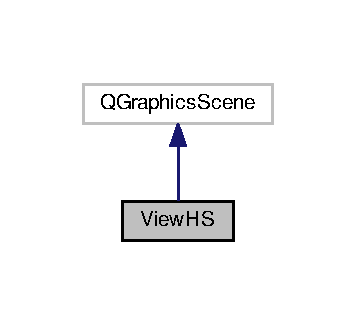
\includegraphics[width=171pt]{classViewHS__inherit__graph}
\end{center}
\end{figure}


Collaboration diagram for View\+H\+S\+:
\nopagebreak
\begin{figure}[H]
\begin{center}
\leavevmode
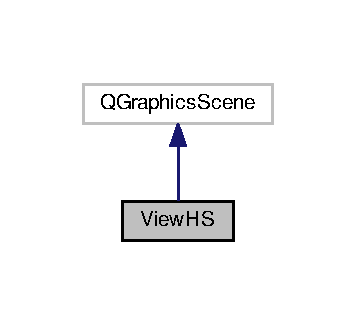
\includegraphics[width=171pt]{classViewHS__coll__graph}
\end{center}
\end{figure}
\subsection*{Public Member Functions}
\begin{DoxyCompactItemize}
\item 
\hypertarget{classViewHS_a823a2ac43ccf8f3f2c1b20e10294b6c4}{\hyperlink{classViewHS_a823a2ac43ccf8f3f2c1b20e10294b6c4}{View\+H\+S} ()}\label{classViewHS_a823a2ac43ccf8f3f2c1b20e10294b6c4}

\begin{DoxyCompactList}\small\item\em Constructor. \end{DoxyCompactList}\item 
void \hyperlink{classViewHS_a6aaa21b53107dc9cbb4c9ebdde2dd713}{clear\+Field} ()
\begin{DoxyCompactList}\small\item\em Clear method. \end{DoxyCompactList}\item 
void \hyperlink{classViewHS_adb138a27be0bf95b1f6647e7e639b48f}{draw\+Text} (std\+::string text)
\begin{DoxyCompactList}\small\item\em Draw method. \end{DoxyCompactList}\item 
\hyperlink{classViewHS}{View\+H\+S} $\ast$ \hyperlink{classViewHS_afa85eb39c82154a4ee539c4681745a21}{get\+View\+Field} ()
\begin{DoxyCompactList}\small\item\em Get method. \end{DoxyCompactList}\end{DoxyCompactItemize}


\subsection{Detailed Description}
Highscore View. 

View for the Highscore inherits from Q\+Graphics\+Scene 

\subsection{Member Function Documentation}
\hypertarget{classViewHS_a6aaa21b53107dc9cbb4c9ebdde2dd713}{\index{View\+H\+S@{View\+H\+S}!clear\+Field@{clear\+Field}}
\index{clear\+Field@{clear\+Field}!View\+H\+S@{View\+H\+S}}
\subsubsection[{clear\+Field}]{\setlength{\rightskip}{0pt plus 5cm}void View\+H\+S\+::clear\+Field (
\begin{DoxyParamCaption}
{}
\end{DoxyParamCaption}
)}}\label{classViewHS_a6aaa21b53107dc9cbb4c9ebdde2dd713}


Clear method. 

Clears the complete Highscore Scene \hypertarget{classViewHS_adb138a27be0bf95b1f6647e7e639b48f}{\index{View\+H\+S@{View\+H\+S}!draw\+Text@{draw\+Text}}
\index{draw\+Text@{draw\+Text}!View\+H\+S@{View\+H\+S}}
\subsubsection[{draw\+Text}]{\setlength{\rightskip}{0pt plus 5cm}void View\+H\+S\+::draw\+Text (
\begin{DoxyParamCaption}
\item[{std\+::string}]{text}
\end{DoxyParamCaption}
)}}\label{classViewHS_adb138a27be0bf95b1f6647e7e639b48f}


Draw method. 

draws piece of text for highscore output 
\begin{DoxyParams}{Parameters}
{\em text} & complete highscore query as string \\
\hline
\end{DoxyParams}
\hypertarget{classViewHS_afa85eb39c82154a4ee539c4681745a21}{\index{View\+H\+S@{View\+H\+S}!get\+View\+Field@{get\+View\+Field}}
\index{get\+View\+Field@{get\+View\+Field}!View\+H\+S@{View\+H\+S}}
\subsubsection[{get\+View\+Field}]{\setlength{\rightskip}{0pt plus 5cm}{\bf View\+H\+S} $\ast$ View\+H\+S\+::get\+View\+Field (
\begin{DoxyParamCaption}
{}
\end{DoxyParamCaption}
)}}\label{classViewHS_afa85eb39c82154a4ee539c4681745a21}


Get method. 

get\+View\+Field \begin{DoxyReturn}{Returns}
\hyperlink{classViewHS}{View\+H\+S} object 
\end{DoxyReturn}


The documentation for this class was generated from the following files\+:\begin{DoxyCompactItemize}
\item 
view\+H\+S.\+h\item 
view\+H\+S.\+cpp\end{DoxyCompactItemize}

%--- End generated contents ---

% Index
\newpage
\phantomsection
\addcontentsline{toc}{chapter}{Index}
\printindex

\end{document}
